\section{Periodic table}
\begin{table}[ht!]
    \centering
    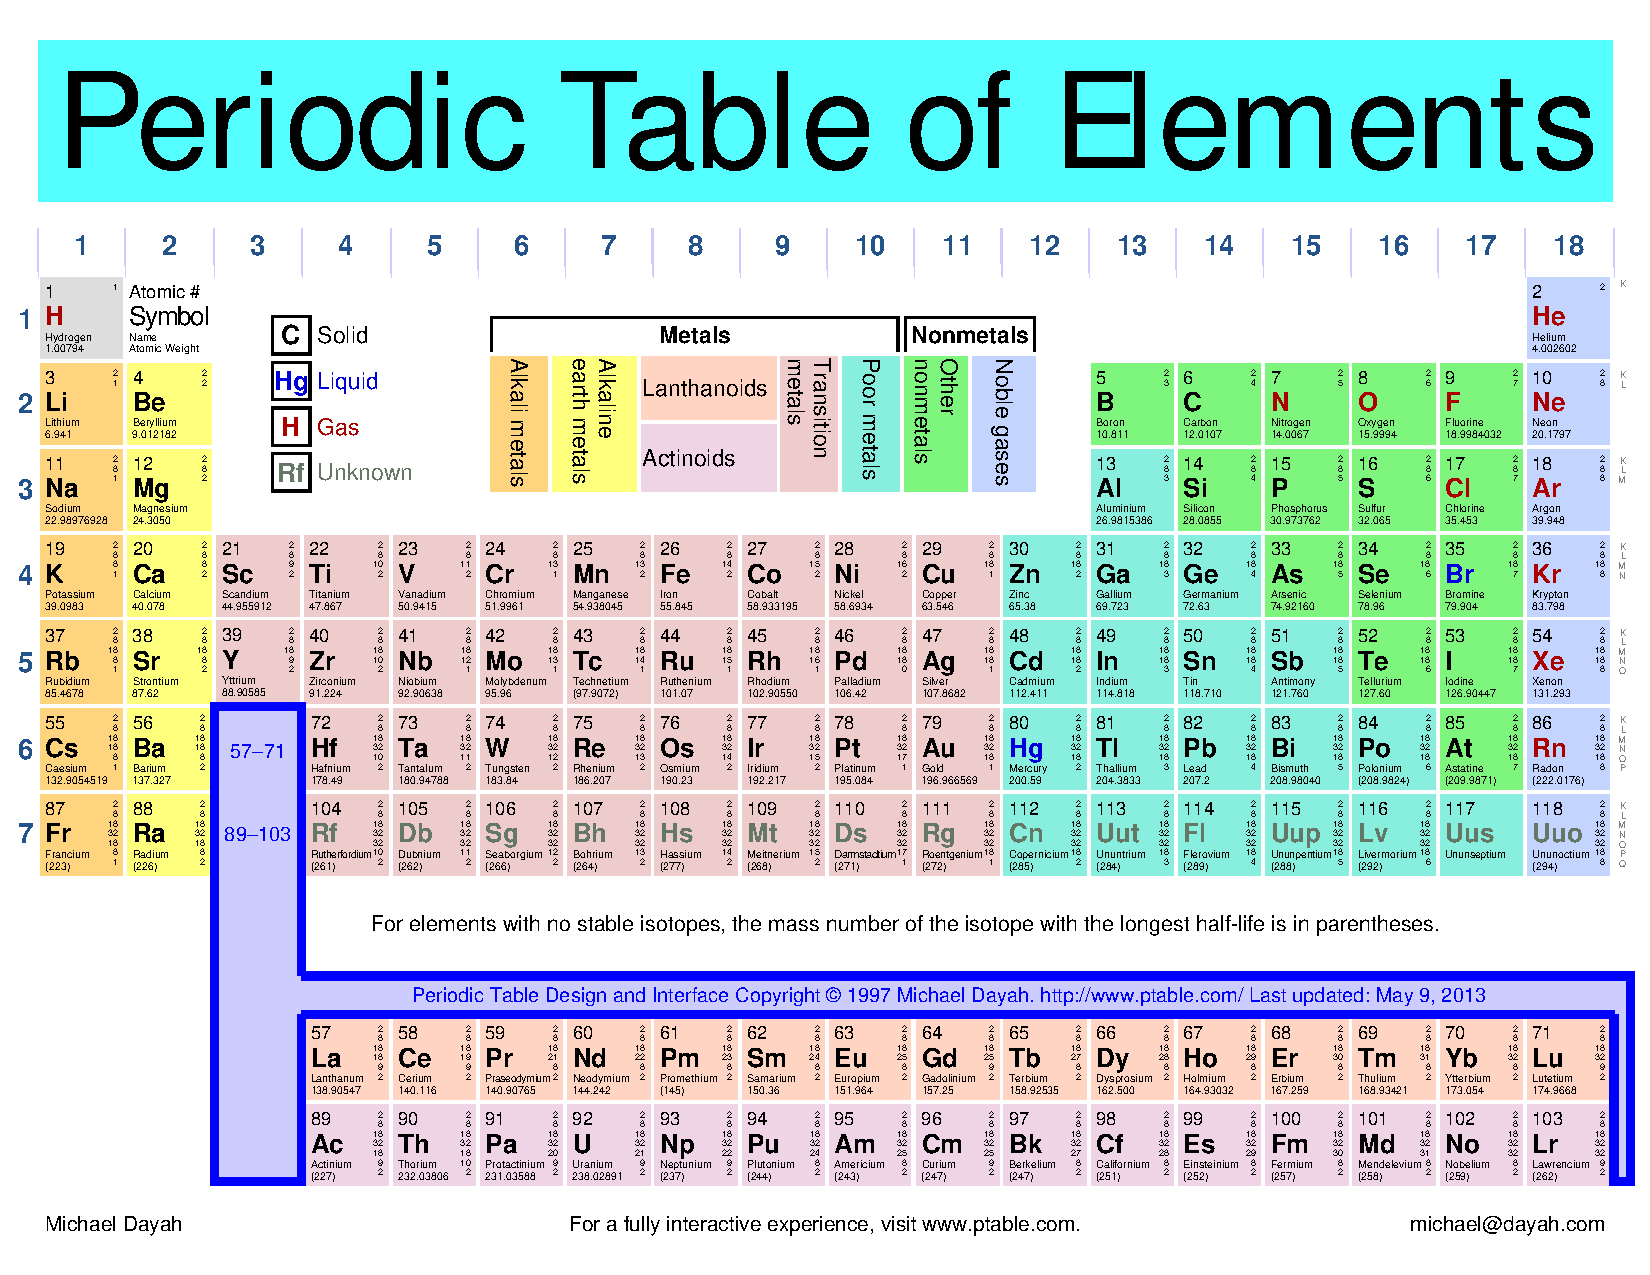
\includegraphics[height=0.9\linewidth,angle=90]{images/Periodic_Table.pdf}
    \caption{The periodic table of elements}
    \label{tab:app_periodictable}
\end{table}

\section{Resistivity and thermal coefficients for various metals}
\begin{table}[ht!]
    \centering
    \begin{tabular}{llll}
    \toprule
        Metal & $\rho_0$ (\si{\nano\ohm\meter}) & $\alpha_0$ (\si{1\per\kelvin}) & n \\ \midrule
        Aluminum, Al & 25.0 & 1/233 & \\
        Antimony, Sb & 38 & 1/196 & \\
        Copper, Cu & 15.7 & 1/232 & 1.15 \\
        Gold, Au & 22.8 & 1/251 & \\
        Indium, In & 78.0 & 1/196 & \\
        Platinum, Pt & 98 & 1/255 & 0.94 \\
        Silver, Ag & 14.6 & 1/244 & 1.11 \\
        Tantalum, Ta & 117 & 1/294 & 0.93 \\
        Tin, Sn & 110 & 1/217 & 1.11 \\
        Tungsten, W & 50 & 1/202 & 1.20 \\
        Iron, Fe & 84.0 & 1/152 & 1.80 \\
        Nickel, Ni & 59.0 & 1/125 & 1.72 \\
    \bottomrule
    \end{tabular} \\
    For non-magnetic metals, $n$ is close to unity.
    \caption{Resistivityand  thermal coefficient of resistivity for various metals}
    \label{app:resistivity}
\end{table}

\section{Hall coefficients}
\begin{table}[ht!]
    \centering
    \begin{tabular}{llll}
    \toprule
        Metal & $n$ (\si{\meter\tothe{-3}}) & $R_H$ (\si{\meter\tothe{3}\per\ampere\second}) & $\mu_h=|\sigma R_H|$ (\si{\square\meter\per\volt\second}) \\ \midrule
            & $\times 10^{28}$ & $\times 10^{-11}$ & $\times 10^{-4}$ \\
        Ag & 5.85 & -9.0 & 57 \\
        Al & 18.06 & -3.5 & 13 \\
        Au & 5.90 & -7.2 & 31 \\
        Be & 24.2 & +3.4 & ? \\
        Cu & 8.45 & -5.5 & 32 \\
        Ga & 15.3 & -6.3 & 3.6 \\
        In & 11.49 & -2.4 & 2.9 \\
        Mg & 8.60 & -9.4 & 22 \\
        Na & 2.56 & -25 & 53 \\
    \bottomrule
    \end{tabular}
    \caption{Hall coefficients of various metals}
    \label{app:Hall}
\end{table}

\section{Thermal conductivity}
\begin{table}[ht!]
    \centering
    \begin{tabular}{llllllll}
    \toprule
        \multicolumn{2}{c}{Pure metals} & \multicolumn{2}{c}{Metal alloys} & \multicolumn{2}{c}{Ceramics} & \multicolumn{2}{c}{Polymersmics} \\\midrule
        Nb & 52 & Stainless steel & 12-16 & Glass-borosilicate & 0.75 & PVC & 0.17 \\
        Fe & 80 & Bronce (95\% Cu - 5\% Sn) & 80 & Alumina (Al$_2$O$_3$) & 30 & Teflon & 0.25 \\
        Al & 250 & Brass (63\% Cu - 37\% Zn) & 125 & Beryllium oxyde & 260 & Polyethylene & 0.4 \\
        Cu & 390 && & Diamond & 1000 && \\
        Ag & 420 && && && \\
    \bottomrule
    \end{tabular}
    \caption{Thermal conductivity $\kappa$ (\si{\watt\per\meter\kelvin}) for various materials}
    \label{app:thermalcond}
\end{table}

\section{Seebeck coefficients}
\begin{table}[ht!]
    \centering
    \begin{tabular}{lllll}
    Metal & S at \SI{0}{\degreeCelsius} (\si{\micro\volt\per\kelvin}) & S at \SI{27}{\degreeCelsius} (\si{\micro\volt\per\kelvin}) & $E_F$ (\si{\eV}) & x \\ \toprule
    Al   & -1.6    & -1.8   & 11.6 & 2.78    \\
    Au  & +1.79 & +1.94 & 5.5   & -1.48  \\
    Cu  & +1.70 & +1.84 & 7.0   & -1.79  \\
    K    &            &  -12.5 & 2.0   & 3.8      \\
    Li   & +14     &           & 4.7    & -9.7    \\
    Mg & -1.3    &           & 7.1    & 1.38     \\
    Na  &            & -5      & 3.1   & 2.2        \\
    Pd  & -9.00   & -9.99 &         &             \\
    Pt  & -4.45    & -5.28 &         &             \\ \bottomrule
    \end{tabular}
    \caption{Seebeck coefficients of selected materials. (Source: Kasap, Table 4.3)}
    \label{app:Seebeck}
\end{table}